\documentclass[10pt,aspectratio=169]{beamer}
\usepackage[utf8]{vietnam}
\usepackage{fil}

\title{Mô phỏng thuật toán Reinforcement Learning cho Serverless}
\subtitle{Future Internet Laboratory}
\author{Nguyễn Phạm Trung Hiếu}
\date{Ngày 5 tháng 5 năm 2024}

\begin{document}

\maketitle

\begingroup
    \begin{frame}{Nội dung chính}{}
        \tableofcontents
    \end{frame}
\endgroup

\section{Nội dung cần chỉnh sửa theo yêu cầu bài toán}

\subsection{Nội dung đã hoàn thành}

\begin{frame}{Nội dung đã hoàn thành}{\secname}
\begin{itemize}
\setlength\itemsep{8pt}
\item Cập nhật thời gian tính reward và đưa ra action thành 10s.
\item Sửa hàm \keyword{\textcolor{mainblue}{\lstinline{_get_request()}}} có chức năng nhận request theo phân phối Poisson thay vì nhận một lượng request cố định.
\item Tạm thời sử dụng công thức tính reward đơn giản = số request đến WarmCPU.
\item Thêm điều kiện kiểm tra xem container nào đang chuyển trạng thái hoặc không:
\begin{itemize}
\setlength\itemsep{4pt}
\item[-] container đang chuyển thì không đưa ra action $ \rightarrow $ chọn action khác.
\item[-] container không chuyển thì đưa ra action bình thường.
\end{itemize}
\item[] $ \longrightarrow $ Thêm ma trận \keyword{\textcolor{mainblue}{\lstinline{_is_changing_matrix}}} với các phần tử 0 là không chuyển trạng thái và 1 là đang chuyển trạng thái.
\end{itemize}
\end{frame}

\subsection{Vấn đề còn lại}

\begin{frame}{Vấn đề còn lại}{\secname}
\begin{itemize}
\setlength\itemsep{8pt}
\item Sửa hàm \keyword{\textcolor{mainblue}{\lstinline{_get_reward()}}} tạm thời bỏ qua công thức tính reward phức tạp, đặt thành:
\begin{equation*}
Reward = n_{request-to-L2} - \alpha \times t_{pending} - \beta \times r
\end{equation*}
trong đó:
\begin{itemize}
\setlength\itemsep{4pt}
\item[-] $ n_{request-to-L2} $ là số request đến WarmCPU là số request được xử lý xong trong khoảng thời gian 10s.
\item[-] $ t_{pending} $ là thời gian chờ là thời gian chuyển trạng thái sang WarmCPU để xử lý request (lưu ý 2-3 trường hợp).
\item[-] $ r $ là tài nguyên sử dụng để đánh giá (RAM, CPU...).
\end{itemize}
\item Đồng bộ về mặt thời gian xử lý song song $ \rightarrow $ Ước tính được request có được xử lý xong hay không, rồi mới đợi một khoảng chờ cho đến khi tính reward.
\end{itemize}
\end{frame}

\begin{frame}{Vấn đề còn lại: Thời gian xử lý song song}{\secname}
Ví dụ, một request được xử lý trong 12s, mô phỏng yêu cầu cứ 10s tính reward một lần:
\begin{center}
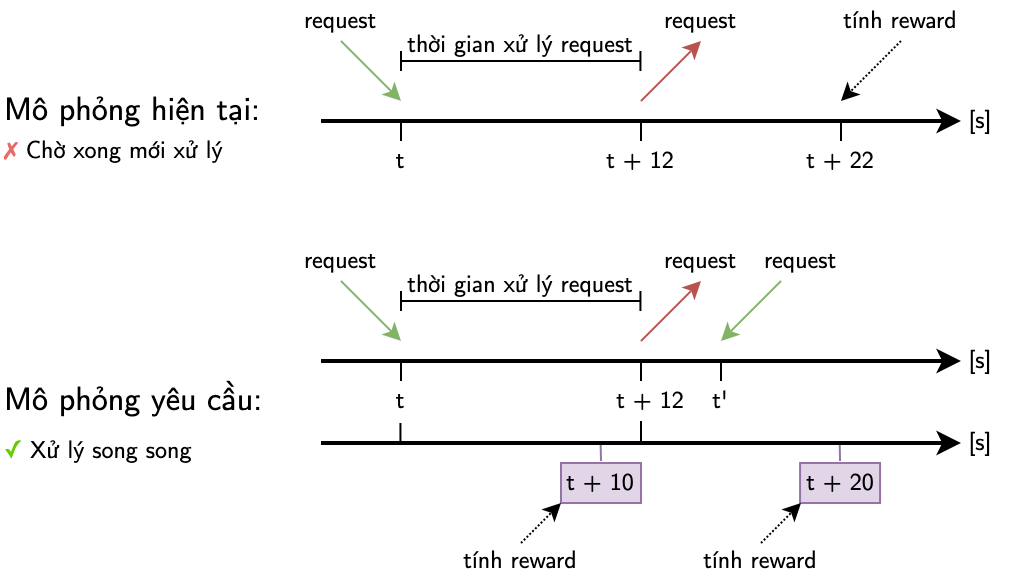
\includegraphics[width=0.64\textwidth]{source/1.png}\\
\end{center}
\end{frame}

\section{Các lưu ý cần nhớ và phát triển}

\begin{frame}{Các lưu ý cần nhớ và phát triển}
\begin{itemize}
\setlength\itemsep{8pt}
\item RAM và tài nguyên sử dụng trong khi chuyển trạng thái không ảnh hưởng.
\item Giả sử hệ thống ban đầu toàn bộ đều ở WarmDisk (thay vì Null như trước).
\item Công thức tính reward ban đầu:
\begin{equation*}
Reward = a \times Profit - b \times Energy_{cost} - Penalty_{delay} - Penalty_{abandone}
\end{equation*}
\item Tìm hiểu và áp dụng phương pháp tính reward theo cập nhật mềm (long term).
\item Cần tăng $ \lambda $ lên khoảng 500 hoặc hơn $ \rightarrow $ đảm bảo hệ thống không quá rảnh.
\end{itemize}
\end{frame}

\section{Kết luận}

\begin{frame}{Kết luận}
\begin{itemize}
\setlength\itemsep{8pt}
\item Link Github mô phỏng: \textit{
\href{https://github.com/owofuyuki/reinforcement-learning-for-serverless}{https://github.com/owofuyuki/reinforcement-learning-for-serverless}}
\item Kết quả mô phỏng chưa đánh giá được vấn đề cho bài toán.
\item Chỉnh sửa mô phỏng...
\end{itemize}
\end{frame}

\backmatter

\end{document}